\documentclass[fullscreen=true, unicode, bookmarks=false]{beamer}
\usepackage[T2A]{fontenc}
\usepackage[utf8]{inputenc}
\usepackage[english, russian]{babel}
\usepackage{amsmath}
\usepackage{amsmath,amsfonts,amssymb}
\usepackage[export]{adjustbox}
\usepackage{textgreek}
\newtheorem{rustheorem}{Теорема }
\sloppy

\DeclareMathOperator{\arsh}{arsh}

\setbeamertemplate{navigation symbols}{}

\usetheme{Madrid}

\usecolortheme{whale}

\usefonttheme{professionalfonts} % default family is serif

\setbeamertemplate{footline}{\hspace*{.5cm}\scriptsize{\insertshorttitle
\hspace*{50pt} \hfill\hspace*{.5cm}}\vspace{5pt}} 

\setbeamercolor{bibliography entry author}{fg=black}

\title[]{ {\huge Устойчивые колебательные решения в цепочках с диффузионным взаимодействием и дополнительной внутренней связью } }   
\author[]{{\large Ивановский Л.И.}} 
\date{ }
\institute[]
{ Ярославль, ЯрГУ им. П.Г Демидова }

\begin{document}

\begin{frame}
\titlepage
\end{frame} 

\begin{frame}
\frametitle{ Цепочка уравнений с диффузионным взаимодействием }
 
\begin{equation}
	\dot u_j = N^2(u_{j+1} - 2u_j + u_{j-1}) + \gamma u_j - u_j^3, \qquad j = \overline{1, N},
\end{equation}

\begin{equation}
	u_0 = u_1, \; u_{N+1} = u_N + \dfrac{\alpha}{N}u_k, \qquad 1 \leqslant k < N,
\end{equation}

\bigskip

$$ u_j = u_j(t), \quad t \geqslant 0, \quad \alpha, \gamma \in \mathbb{R}. $$

\bigskip
\pause

\begin{figure} 
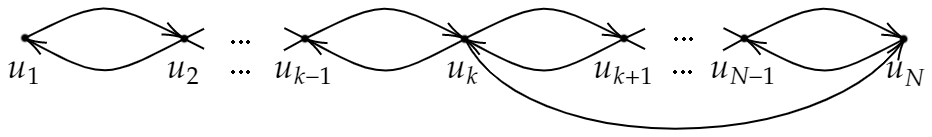
\includegraphics[scale=0.47]{u_j.png}  
\end{figure}

\end{frame}

\begin{frame}
\frametitle{ Линеаризованная в нуле система уравнений }
 
\begin{equation}
	\dot{u}_j =  N^2(u_{j+1} - 2u_j + u_{j-1}) + \gamma u_j, \qquad j = \overline{1, N},
\end{equation}

\bigskip

\begin{equation}
	u_0 = u_1, \quad u_{N+1} = u_N + \dfrac{\alpha}{N}u_k, \qquad 1 \leqslant k < N,
\end{equation}

\end{frame}

\begin{frame}
\frametitle{ Построение характеристического уравнения }
 
$$ u_j = e^{\lambda t} \ch \delta x_j, $$

$$ x_j = -\dfrac{1}{2N} + \dfrac{j}{N}. $$

\bigskip
\pause

\begin{itemize}

\item { $ j \leqslant N-1: $ 
}
\begin{equation}
\delta = 2N \arsh \dfrac{\sqrt{-\gamma+\lambda}}{2N}.
\end{equation}
\medskip
\pause
\item { $ j = N: $ 
}
\begin{equation}
\alpha = \dfrac{\sqrt{-\gamma+\lambda}\sh\delta}{\ch\delta x_k}.
\end{equation}

\end{itemize}

\end{frame}

\begin{frame}
\frametitle{ Потеря устойчивости нулевого решения }

\begin{itemize}

\item { $ \lambda = 0: $ 
}

\begin{equation}
\alpha_u = \frac{ \sqrt{-\gamma} \, \sh \delta_u }{ \ch\delta_u x_k },.
\end{equation}
$$ \delta_u = 2N \arsh \dfrac{\sqrt{-\gamma}}{2N} $$

\medskip
\pause

\item { $ \lambda = \pm i \omega: \; $ 
}

\begin{equation}
\alpha_c = \frac{ \sqrt{-\gamma + i \omega} \, \sh \delta_c }{ \ch\delta_c x_k }, 
\end{equation}
$$ \delta_c = 2N \arsh \dfrac{\sqrt{-\gamma + i \omega}}{2N}. $$

\end{itemize}

\bigskip
\pause

$$ N = 50. $$	

\end{frame}

\begin{frame}
\frametitle{ Предельный случай }

$$ N \rightarrow \infty: \qquad \delta \rightarrow \sqrt{-\gamma + \lambda}. $$

\bigskip
\pause

\begin{equation}
	\dot{u} = u'' + \gamma u - u^3,	
\end{equation}
\begin{equation}
	u'(0, t) \, = 0, \qquad u'(1, t) \, = \alpha\,u(x_0, t),
\end{equation}

\smallskip

$$ x \in [0,1] ,\quad  x_0 \in [0, 1). $$

\bigskip
\pause

\begin{equation}
\alpha = \dfrac{\sqrt{-\gamma+\lambda}\sh\sqrt{-\gamma+\lambda}}{\ch\sqrt{-\gamma+\lambda}\:x_0}.
\end{equation}

\end{frame}

\begin{frame}
\frametitle{ Критические зависимости $ \alpha_{cr}(\gamma), \; 1 \leqslant k \leqslant 17 $ }

\begin{figure} 
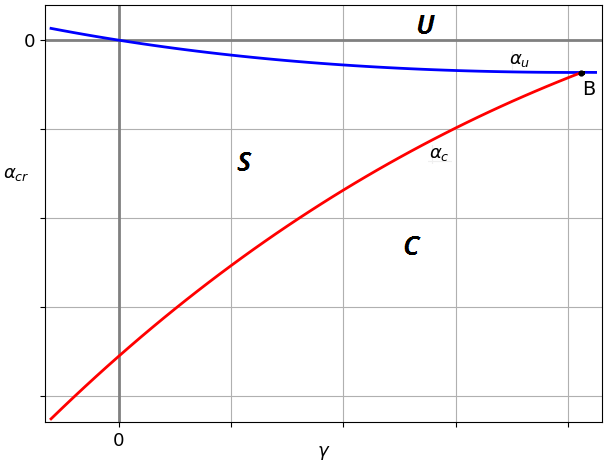
\includegraphics[scale=0.59]{scheme0117.png}  
\end{figure}
$$ B=(\gamma_*, \alpha_*) $$

\end{frame}

\begin{frame}
\frametitle{ Критические зависимости $ \alpha_{cr}(\gamma), \; k = 1 $ }

\begin{figure} 
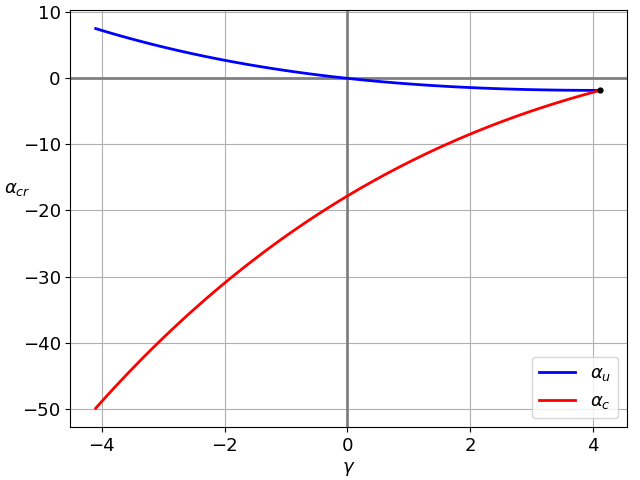
\includegraphics[scale=0.55]{alphas_000.png}  
\end{figure}
$$ \gamma_* \approx 4.116 $$

\end{frame}

\begin{frame}
\frametitle{ Критические зависимости $ \alpha_{cr}(\gamma), \; k = 17 $ }

\begin{figure} 
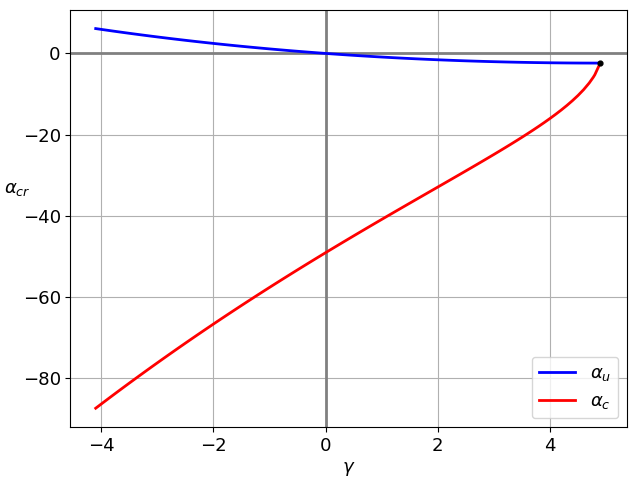
\includegraphics[scale=0.55]{alphas_033.png}  
\end{figure}
$$ \gamma_* \approx 4.896 $$

\end{frame}

\begin{frame}
\frametitle{ Критические зависимости $ \alpha_{cr}(\gamma), \; 18 \leqslant k \leqslant 23 $ }

\begin{figure} 
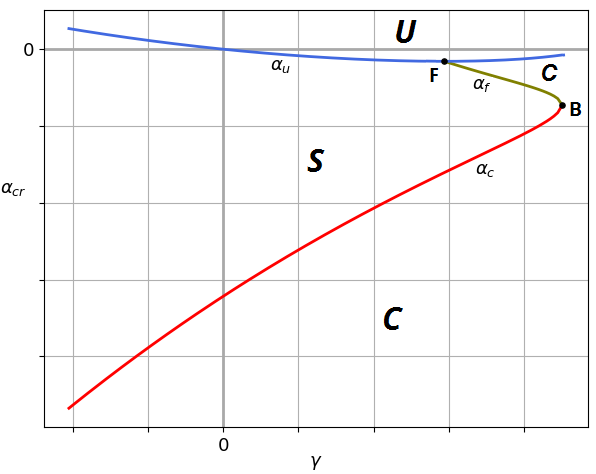
\includegraphics[scale=0.55]{scheme1823.png}  
\end{figure}
$$ F = (\overline{\gamma}, \overline{\alpha}) $$

\end{frame}

\begin{frame}
\frametitle{ Критические зависимости $ \alpha_{cr}(\gamma), \; k = 20 $ }

\begin{figure} 
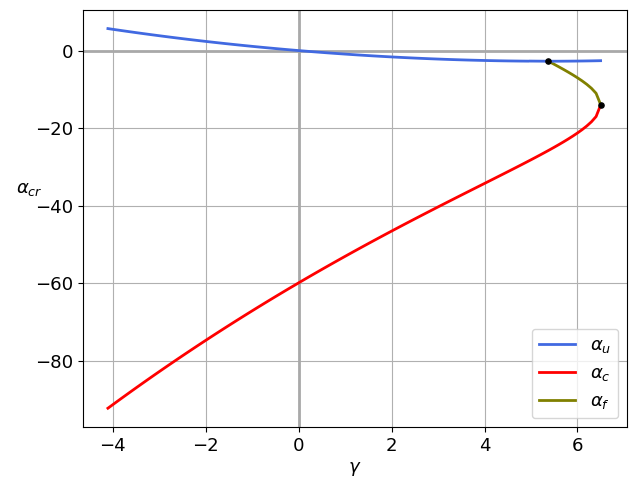
\includegraphics[scale=0.55]{alphas_039.png}  
\end{figure}
$$ \overline{\gamma} \approx 5.375, \quad \gamma_* \approx 6.497 $$

\end{frame}

\begin{frame}
\frametitle{ Критические зависимости $ \alpha_{cr}(\gamma), \; k = 23 $ }

\begin{figure} 
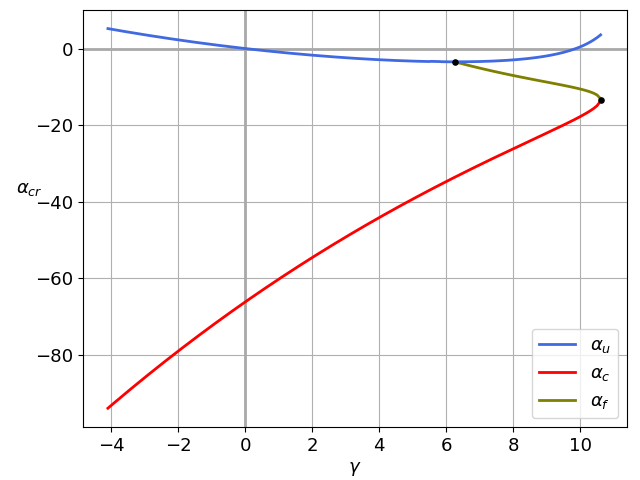
\includegraphics[scale=0.55]{alphas_045.png}  
\end{figure}
$$ \overline{\gamma} \approx 6.258, \quad \gamma_* \approx 10.608 $$

\end{frame}

\begin{frame}
\frametitle{ Критические зависимости $ \alpha_{cr}(\gamma), \; k = 24 $ }

\begin{figure} 
\begin{minipage}[h]{0.49\linewidth}
\begin{center}
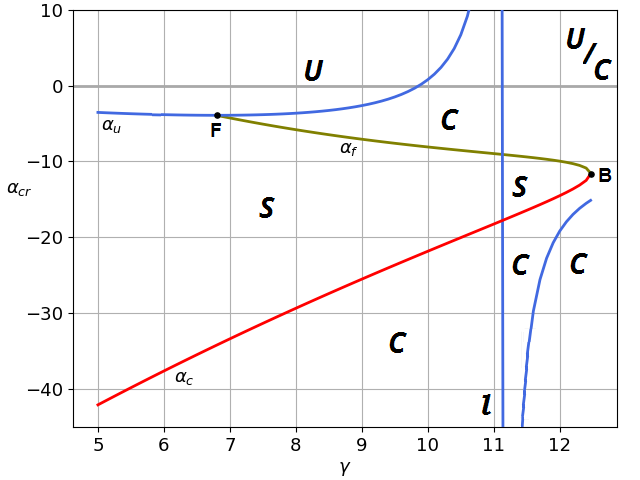
\includegraphics[scale=0.37]{scheme24.png} 
\end{center}
\end{minipage} 
\hfill
\begin{minipage}[h]{0.49\linewidth}
\begin{center}
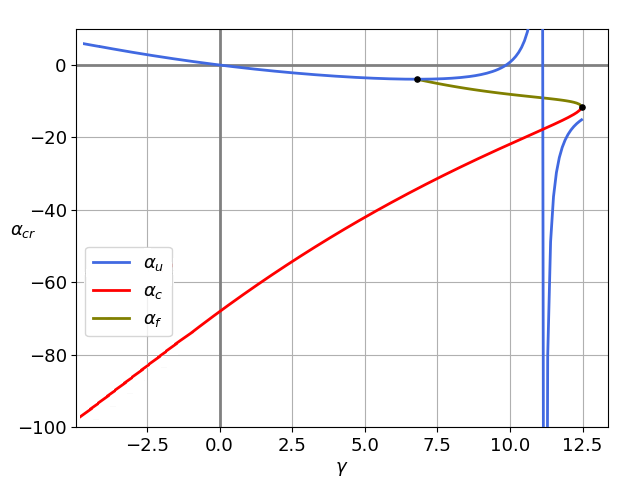
\includegraphics[scale=0.37]{alphas_047.png}
\end{center}
\end{minipage} 
\end{figure}

$$ \overline{\gamma} \approx 6.796, \quad l \approx 9.486, \quad \gamma_* \approx 12.467 $$

\end{frame}

\begin{frame}
\frametitle{ Критические зависимости $ \alpha_{cr}(\gamma), \; k = 25 $ }

\begin{figure} 
\begin{minipage}[h]{0.49\linewidth}
\begin{center}
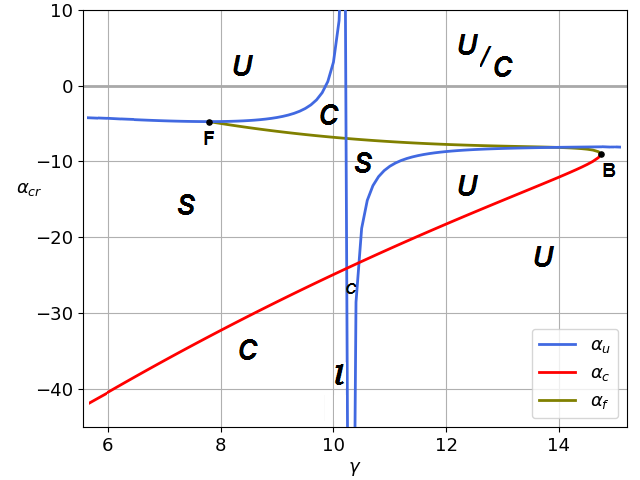
\includegraphics[scale=0.36]{scheme25.png} 
\end{center}
\end{minipage} 
\hfill
\begin{minipage}[h]{0.49\linewidth}
\begin{center}
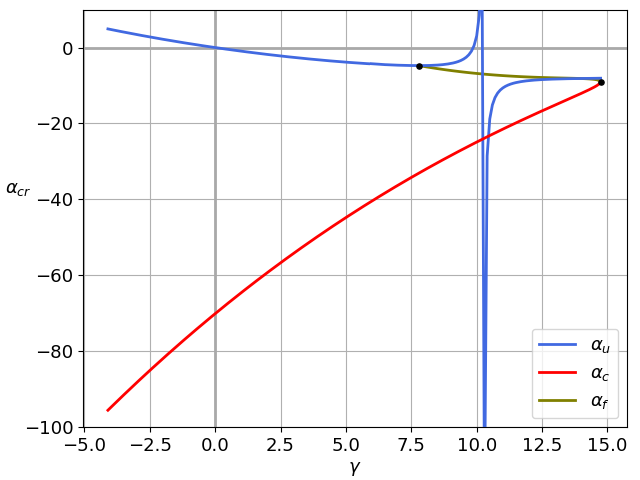
\includegraphics[scale=0.36]{alphas_049.png}
\end{center}
\end{minipage} 
\end{figure}

$$ \overline{\gamma} \approx 7.794, \quad l \approx 10.277, \quad \gamma_* \approx 14.738 $$

\end{frame}

\begin{frame}
\frametitle{ Критические зависимости $ \alpha_{cr}(\gamma), \; 26 \leqslant k \leqslant 32 $ }

\begin{figure} 
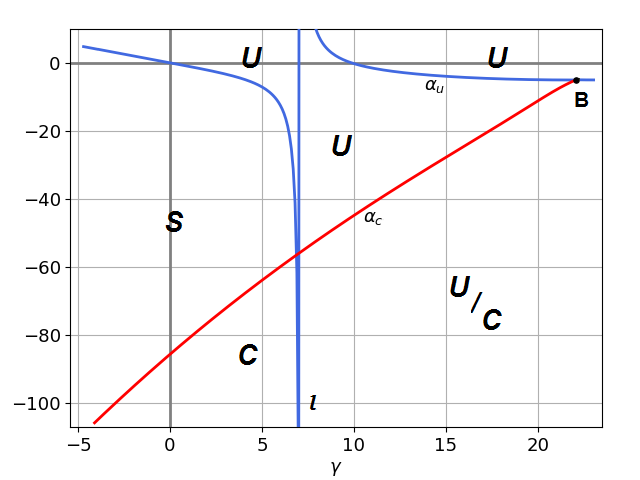
\includegraphics[scale=0.59]{scheme2632.png}  
\end{figure}

\end{frame}

\begin{frame}
\frametitle{ Критические зависимости $ \alpha_{cr}(\gamma), \; k = 26 $ }

\begin{figure} 
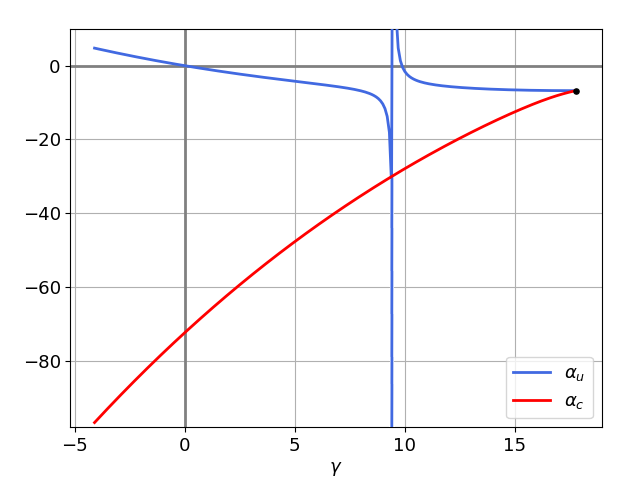
\includegraphics[scale=0.55]{alphas_051.png}  
\end{figure}
$$ l \approx 9.486, \quad \gamma_* \approx 17.763 $$

\end{frame}

\begin{frame}
\frametitle{ Критические зависимости $ \alpha_{cr}(\gamma), \; k = 32 $ }

\begin{figure} 
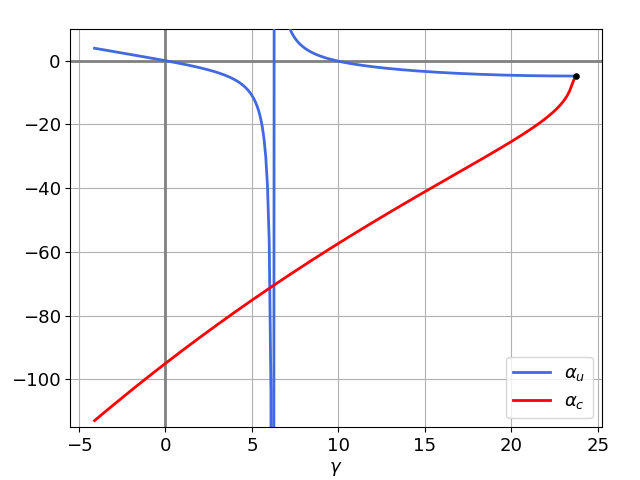
\includegraphics[scale=0.55]{alphas_063.png}  
\end{figure}
$$ l \approx 6.217, \quad \gamma_* \approx 23.717 $$

\end{frame}

\begin{frame}
\frametitle{ Критические зависимости $ \alpha_{cr}(\gamma), \; 33 \leqslant k \leqslant 38 $ }

\begin{figure} 
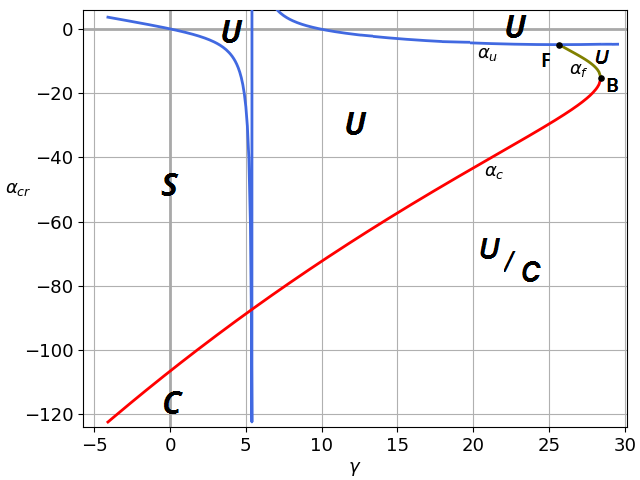
\includegraphics[scale=0.59]{scheme3338.png}  
\end{figure}

\end{frame}

\begin{frame}
\frametitle{ Критические зависимости $ \alpha_{cr}(\gamma), \; k = 34 $ }

\begin{figure} 
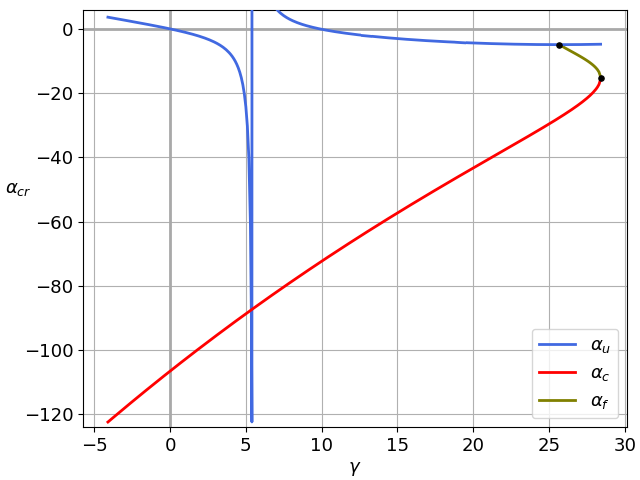
\includegraphics[scale=0.55]{alphas_067.png}  
\end{figure}
$$ l \approx 5.496, \quad \overline{\gamma} \approx 25.682, \quad \gamma_* \approx 28.407 $$

\end{frame}

\begin{frame}
\frametitle{ Критические зависимости $ \alpha_{cr}(\gamma), \; k = 38 $ }

\begin{figure} 
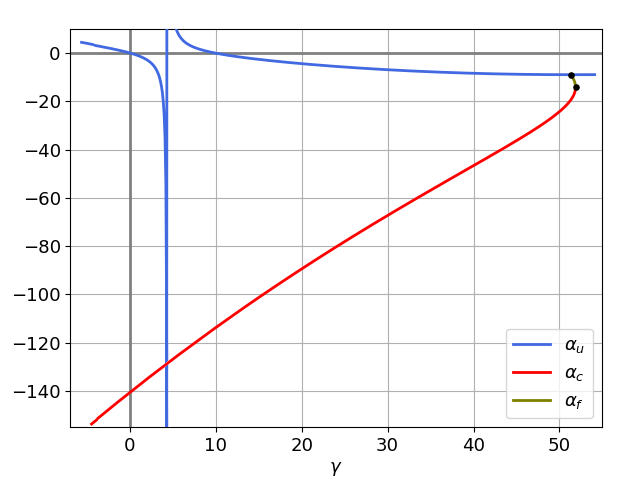
\includegraphics[scale=0.55]{alphas_075.png}  
\end{figure}
$$ l \approx 4.386, \quad \overline{\gamma} \approx 51.305, \quad \gamma_* \approx 51.873 $$

\end{frame}

\begin{frame}
\frametitle{ Критические зависимости $ \alpha_{cr}(\gamma), \; 39 \leqslant k \leqslant 50 $ }

\begin{figure} 
\begin{minipage}[h]{0.49\linewidth}
\begin{center}
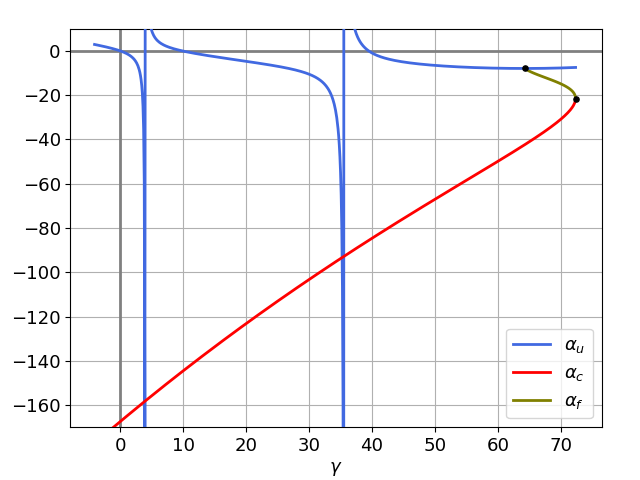
\includegraphics[scale=0.37]{alphas_079.png} \\ (а) $ k = 40, \quad \gamma_* \approx 72.359 $
\end{center}
\end{minipage} 
\hfill
\begin{minipage}[h]{0.49\linewidth}
\begin{center}
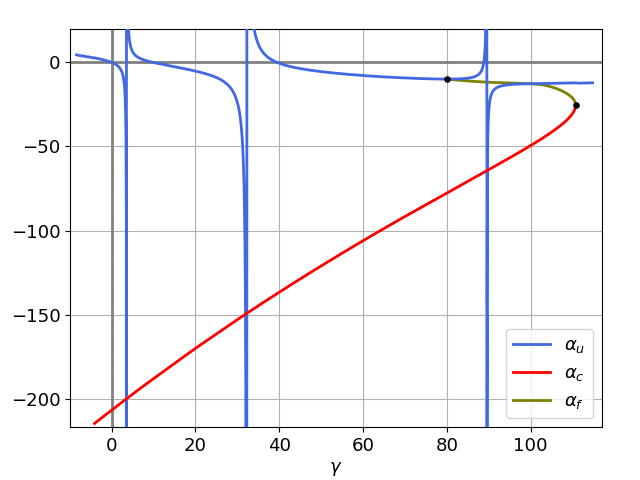
\includegraphics[scale=0.37]{alphas_083.png} \\ (б) $ k = 42, \quad \gamma_* \approx 110.74 $
\end{center}
\end{minipage} 
\end{figure}

\end{frame}

\begin{frame}

\begin{rustheorem}
Для линеаризованной системы (3), (4) критические зависимости, рассчитываемые по формулам (7), (8), позволяют получить три области параметров $ (\alpha,\: \gamma) $: $ S $, для случая устойчивого нулевого решения, $ U $ -- для случая двух устойчивых состояний равновесия, симметрично ответвляющихся от нулевого решения и области $ C $, в которой наблюдается возникновение устойчивого цикла в окрестности нулевого состояния равновесия.
\end{rustheorem}

\end{frame}

\begin{frame}
\frametitle{ Локальный анализ системы }

\begin{equation}
	u_j = \sqrt{\varepsilon}u_{j,0} + \varepsilon u_{j,1} + \varepsilon^{\frac{3}{2}} u_{j,2} + O(\varepsilon^2), \qquad j = \overline{1, N}.
\end{equation}

\bigskip

$$ u_j = u_j(s), \quad s = \varepsilon t, $$

$$ \varepsilon = | \alpha - \alpha_{cr} |, \quad \varepsilon \ll 1.  $$

\end{frame}

\begin{frame}
\frametitle{ Случай дивергентной потери устойчивости }

\begin{itemize}
\item { $ \lambda = 0: \quad \varepsilon=\alpha-\alpha_u, $
}
\end{itemize}

\bigskip
\pause

\begin{equation}
	\dot u_{j,0} = N^2(u_{j+1,0} - 2u_{j,0} + u_{j-1,0}) + \gamma u_{j,0},
\end{equation}
\begin{equation}
	u_{0,0} = u_{1,0}, \quad u_{N+1,0} = u_{N,0} + \dfrac{\alpha_u}{N}u_{k,0}, \qquad 1 \le k < N
\end{equation}

\bigskip

$$ u_{j,0} = \rho(s) \ch \delta_u x_j, $$

\bigskip

$$ \alpha_u = \frac{ \sqrt{-\gamma} \, \sh \delta_u }{ \ch\delta_u x_k }, \quad \delta_u = 2N \arsh \dfrac{\sqrt{-\gamma}}{2N}, \quad x_j = -\dfrac{1}{2N} + \dfrac{j}{N}. $$

\end{frame}

\begin{frame}
\frametitle{ Случай дивергентной потери устойчивости }

\begin{equation}
	\dot u_{j,2} + \frac{\partial u_{j,0}}{\partial s} = N^2(u_{j+1,2} - 2u_{j,2} + u_{j-1,2}) + \gamma u_{j,2} - u_{j,2}^3,
\end{equation}
\begin{equation}
	u_{0,2} = u_{1,2}, \quad u_{N+1,2} = u_{N,2} + \dfrac{\alpha_u}{N}u_{k,0},
\end{equation}

\bigskip

$$ u_{j,2} = \ch \delta_u x_j. $$

\end{frame}

\begin{frame}
\frametitle{ Случай дивергентной потери устойчивости }

\begin{equation}
	\rho' = \phi_0 \rho + d_0 \rho^3,
\end{equation}

\bigskip

\begin{equation}\label{phi0_div}
\phi_0 = \frac{ 2 \delta_u \ch \delta_u x_k }{ \delta_u \ch \delta_u +\sh \delta_u - \alpha_u x_k \sh \delta_u x_k },
\end{equation}

\begin{equation}\label{d0_div}
d_0 = \frac{ 3\delta_u^2 \sh 3\delta_u - \alpha_u \delta_u \ch 3\delta_u x_k }{ 16( \delta_u \ch \delta_u +\sh \delta_u - \alpha_u x_k \sh \delta_u x_k ) } - \frac{3}{4}.
\end{equation}

\end{frame}

\begin{frame}
\frametitle{ Графики $ \phi_0(\gamma) $ и $ d_0(\gamma) $ }

\begin{figure} 
\begin{minipage}[h]{0.49\linewidth}
\begin{center}
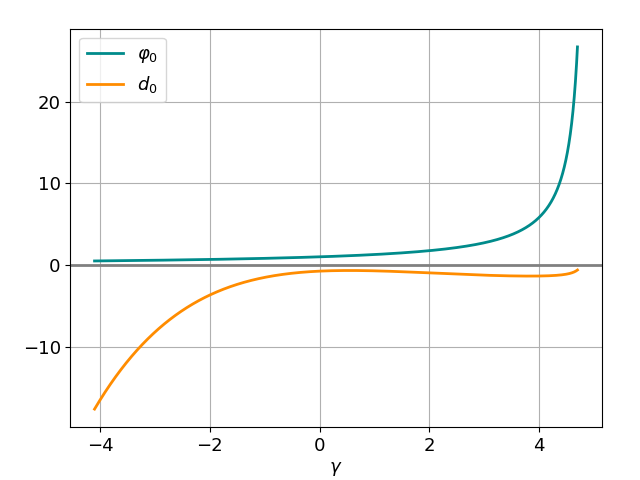
\includegraphics[scale=0.39]{divergent_phi0d0_033.png} \\ (а) $ k=17 $
\end{center}
\end{minipage} 
\hfill
\begin{minipage}[h]{0.49\linewidth}
\begin{center}
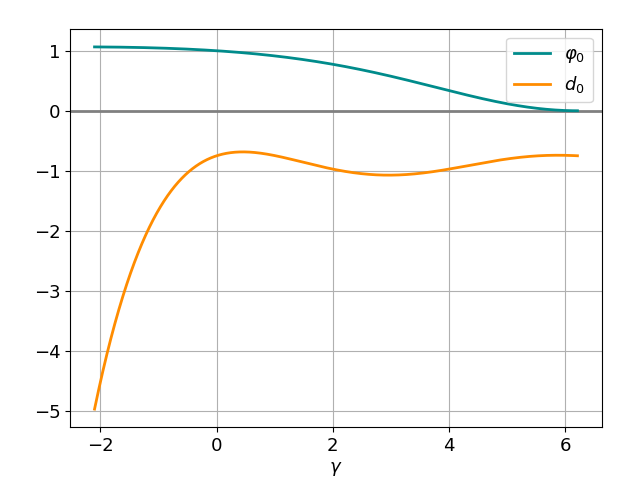
\includegraphics[scale=0.39]{divergent_phi0d0_063.png}  \\ (б) $ k=32 $
\end{center}
\end{minipage} 
\end{figure}

\end{frame}

\begin{frame}
\frametitle{ Графики $ d_0(\gamma) $ }

\begin{figure} 
\begin{minipage}[h]{0.49\linewidth}
\begin{center}
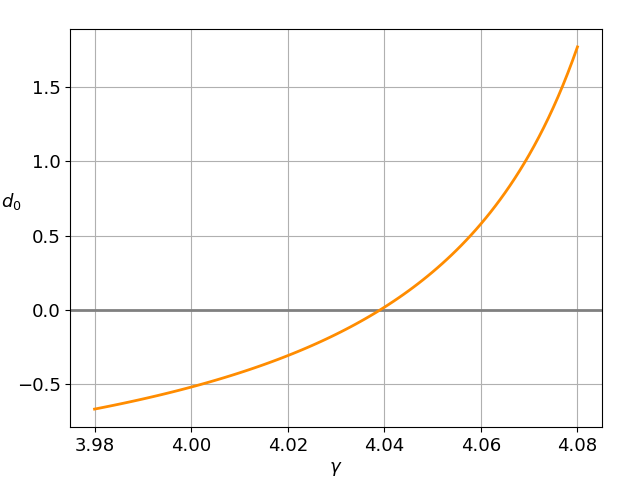
\includegraphics[scale=0.39]{divergent_d0_000.png} \\ (а) $ k=1, \quad \gamma_*\approx 4.116 $
\end{center}
\end{minipage} 
\hfill
\begin{minipage}[h]{0.49\linewidth}
\begin{center}
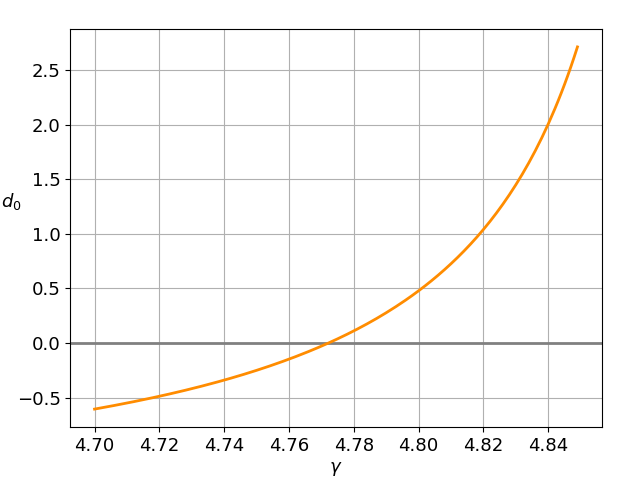
\includegraphics[scale=0.39]{divergent_d0_033.png}  \\ (б) $ k=17, \quad \gamma_*\approx 4.896 $
\end{center}
\end{minipage} 
\end{figure}

\end{frame}

\begin{frame}
\frametitle{ Графики $ d_0(\gamma) $ }

\begin{figure} 
\begin{minipage}[h]{0.49\linewidth}
\begin{center}
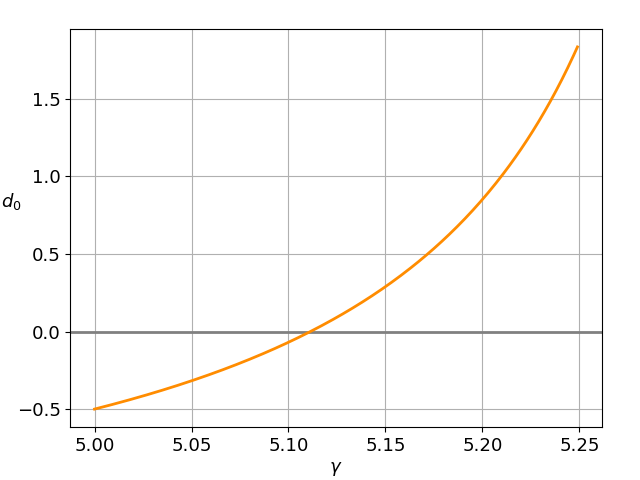
\includegraphics[scale=0.39]{divergent_d0_039.png} \\ (а) $ k=20, \quad \overline{\gamma}\approx 5.375 $
\end{center}
\end{minipage} 
\hfill
\begin{minipage}[h]{0.49\linewidth}
\begin{center}
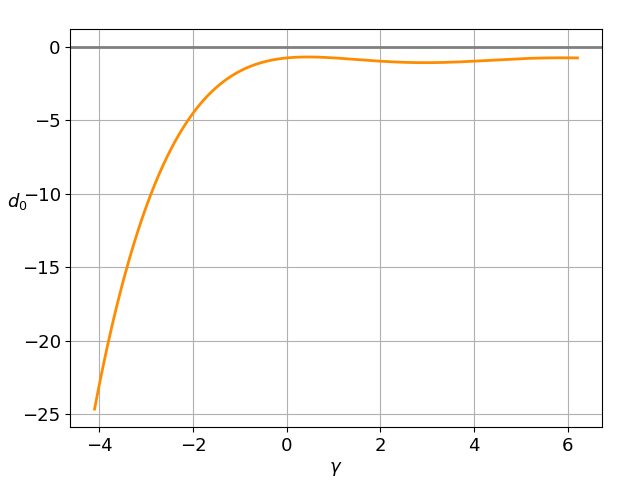
\includegraphics[scale=0.39]{divergent_d0_063.png}  \\ (б) $ k=32, \quad l \approx 6.217 $
\end{center}
\end{minipage} 
\end{figure}

\end{frame}

\begin{frame}
\frametitle{ Случай колебательной потери устойчивости }

\begin{itemize}
\item { $ \lambda = \pm i \omega: \quad \varepsilon=\alpha_c-\alpha, $
}
\end{itemize}

\bigskip
\pause

\begin{equation}
	\dot u_{j,0} = N^2(u_{j+1,0} - 2u_{j,0} + u_{j-1,0}) + \gamma u_{j,0},
\end{equation}
\begin{equation}
	u_{0,0} = u_{1,0}, \quad u_{N+1,0} = u_{N,0} + \dfrac{\alpha_c}{N}u_{k,0}, \qquad 1 \le k < N
\end{equation}

\bigskip

$$ u_{j,0} = z(s) e^{i \omega t} \ch \delta_c x_j + \overline{z(s)} e^{-i \omega t} \overline{\ch \delta_c x_j}, $$

\bigskip

$$ \alpha_c = \frac{ \sqrt{-\gamma + i \omega} \, \sh \delta_c }{ \ch\delta_c x_k }, \quad \delta_c = 2N \arsh \dfrac{\sqrt{-\gamma + i \omega}}{2N}, \quad x_j = -\dfrac{1}{2N} + \dfrac{j}{N}. $$

\end{frame}

\begin{frame}
\frametitle{ Случай колебательной потери устойчивости }

\begin{equation}
	\dot u_{j,2} + \frac{\partial u_{j,0}}{\partial s} = N^2(u_{j+1,2} - 2u_{j,2} + u_{j-1,2}) + \gamma u_{j,2} - u_{j,2}^3,
\end{equation}
\begin{equation}
	u_{0,2} = u_{1,2}, \quad u_{N+1,2} = u_{N,2} + \dfrac{\alpha_c}{N}u_{k,0}, \qquad 1 \le k < N,
\end{equation}

\bigskip

$$ u_{j,2} = e^{i \omega t} \ch \delta_c x_j. $$

\end{frame}

\begin{frame}
\frametitle{ Случай колебательной потери устойчивости }

\begin{equation}
	z' = \phi_0 z + d_0 z |z|^2,
\end{equation}

\bigskip

$$ \phi_0 = -\mbox{Re} \left(\dfrac{2 \delta_c \ch \delta_c x_k}{\delta_c\ch \delta_c + \sh \delta_c - \alpha_c x_k \sh \delta_c x_k} \right), $$

$$ d_0 = \mbox{Re} \left( \dfrac{3 \delta_c (G(\chi) + G(\eta) + 2G(\overline{\delta_c}) )}{2(\delta_c\ch \delta_c + \sh \delta_c - \alpha_c x_k \sh \delta_c x_k)} \right), $$

\bigskip
\pause

$$ \chi = \delta_c + 2 \mbox{Re}\,\delta_c, \qquad \eta = \delta_c + 2 \mbox{Im}\,\delta_c, $$

$$ G(a) = \dfrac{\alpha_c \ch a x_k - a \sh a}{a^2 - \delta_c^2}. $$

\end{frame}

\begin{frame}
\frametitle{ Графики $ \phi_0(\gamma) $ и $ d_0(\gamma), \; k = 1 $ для $ \alpha_{cr}=\alpha_c $ }

\begin{figure} 
\begin{minipage}[h]{0.49\linewidth}
\begin{center}
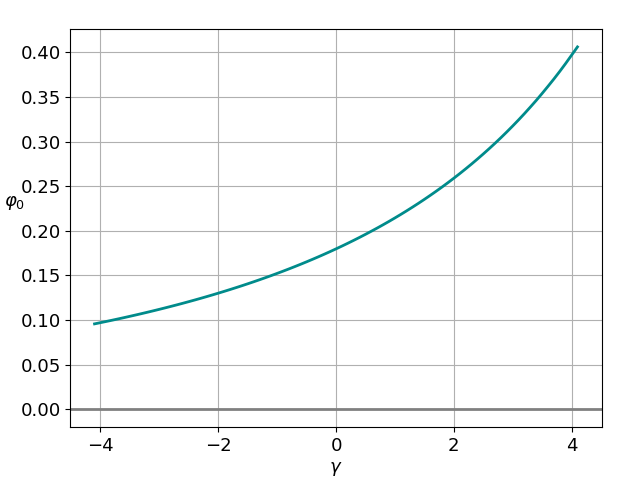
\includegraphics[scale=0.37]{oscillating_phi0_000.png}
\end{center}
\end{minipage} 
\hfill
\begin{minipage}[h]{0.49\linewidth}
\begin{center}
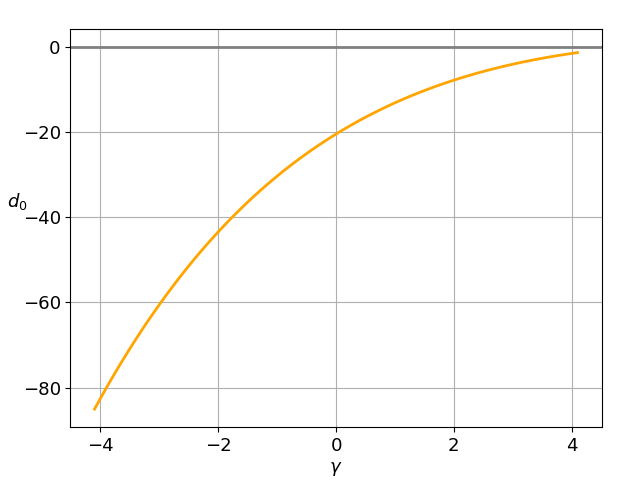
\includegraphics[scale=0.37]{oscillating_d0_000.png} 
\end{center}
\end{minipage} 
\end{figure}

\end{frame}

\begin{frame}
\frametitle{ Графики $ \phi_0(\gamma) $ и $ d_0(\gamma), \; k = 17 $ для $ \alpha_{cr}=\alpha_c $ }

\begin{figure} 
\begin{minipage}[h]{0.49\linewidth}
\begin{center}
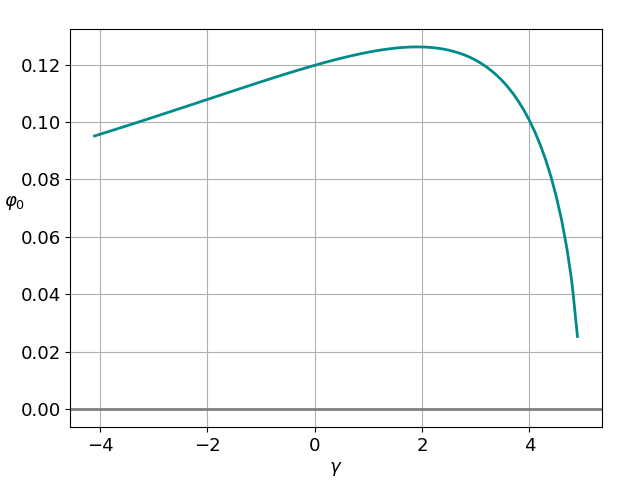
\includegraphics[scale=0.37]{oscillating_phi0_033.png}
\end{center}
\end{minipage} 
\hfill
\begin{minipage}[h]{0.49\linewidth}
\begin{center}
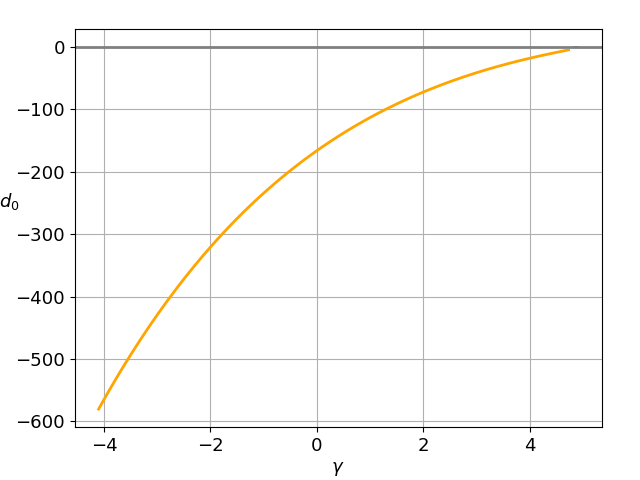
\includegraphics[scale=0.37]{oscillating_d0_033.png} 
\end{center}
\end{minipage} 
\end{figure}

\end{frame}

\begin{frame}
\frametitle{ Графики $ \phi_0(\gamma) $ и $ d_0(\gamma), \; k = 24 $ для $ \alpha_{cr}=\alpha_f $ }

\begin{figure} 
\begin{minipage}[h]{0.49\linewidth}
\begin{center}
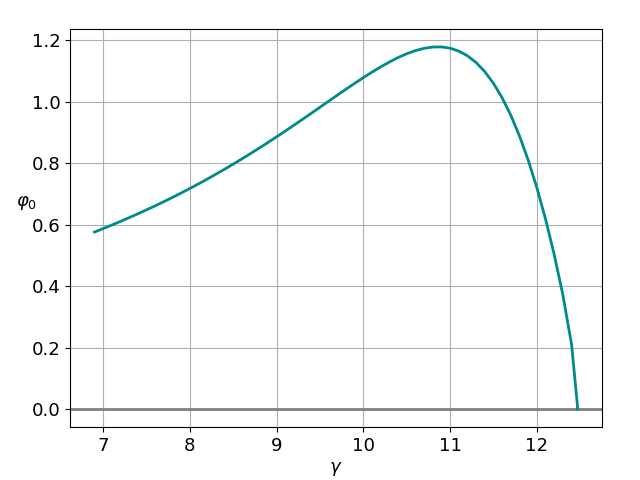
\includegraphics[scale=0.37]{oscillating_phi0_after_tangent_047.png}
\end{center}
\end{minipage} 
\hfill
\begin{minipage}[h]{0.49\linewidth}
\begin{center}
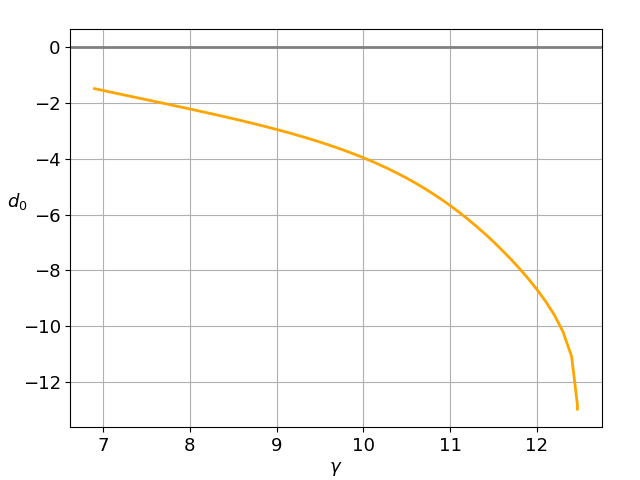
\includegraphics[scale=0.37]{oscillating_d0_after_tangent_047.png} 
\end{center}
\end{minipage} 
\end{figure}

\end{frame}

\begin{frame}

\begin{rustheorem}
Для системы дифференциальных уравнений (1), (2) $\exists\;\Gamma_u\leqslant\gamma_*: \; \gamma<\Gamma_u$ нулевое состояние равновесия теряет свою устойчивость дивергентным способом.
\end{rustheorem}

\bigskip
\pause
\bigskip

\begin{rustheorem}
Для сиcтемы дифференциальных уравнений (1), (2) $\exists\;\Gamma_c\leqslant\gamma_*: \; \gamma<\Gamma_c$ нулевое состояние равновесия теряет свою устойчивость колебательным способом.
\end{rustheorem}

\end{frame}

\begin{frame}
\titlepage
\end{frame}

\end{document}